\documentclass{article}
\usepackage{graphicx}
\usepackage{subfig}
\usepackage{amsmath}
\begin{document}
\section{Related Works} 
\subsection{Preliminaries}
\subsubsection{Motivation: Data Integrity Threat Model for Processor-Memory Architecture}
In the scenario of processor-memory architecture, data integrity refers to maintaining the data on the transmission outside the chip and stored on off-chip memory untampered. If the data stored on off-chip memory , or some external data injected to the system S, we can say that the data integrity of S is attacked. If the system S can not examine the tampered data or injected data, the attack is assumed to be successful. According to our knowledge, there are two aspects of attacks on data integrity:
\begin{itemize}
	\item Introducing new content: The content of data in the system is modified, or data construct by the attacker is inserted to the system.
	\item Replacing data with valid copy: The data D in transmission or on the memory is replace with the following two types of copy: A copy of D at an old time point or a copy of other data from different memory address.
\end{itemize}

\subsubsection{Protection of Integrity: Theoretical Models}
The goal of integrity protection can be defined as the capability to examine whether the data to read by processor has been tampered. According to our knowledge, there are three common types of cryptographic primitives aiming to protect the data integrity of a system, which are cryptographic hash function, Message Authentication Code(MAC) scheme and block-level Added Redundancy Explicit Authentication (AREA). These theoretical models for integrity protection is also called Authentication Primitives(AP) in some research works.

\paragraph{Cryptographic Hash Functions}
Hash is a short message block computed by hash function with data block D as input.
When processor writes a data block to a memory address, the data block D is sent to Hash function and a Hash value H1 is computed and stored on the chip. The hash value H is stored on chip following the order of data block on the memory. The message stored on the memory from chip is data block D alone.
When the processor wants to read a data block D from memory, D is sent to hash function and an hash value H2 is computed. If H1 is identical to H2, then the data block D is assumed to be untampered and read by processor.

Figure 3-a expresses functionality of hash function in integrity protection.
If the integrity of a processor-memory system is protected by hash function, the possible attacks are:
\begin{enumerate}
	\item Modify the content of a data block
	\item Insert new data
	\item Replace the content of a data block with a copy of data from other address
\end{enumerate}
If using hash function to protect integrity, the three attacks in the above list can be defended if the hash function behave like an theoretical random function, which means for any input data block D, its hash value H is randomly assigned.

\paragraph{Message Authentication Code(MAC) Schemes}
\begin{figure}[htbp]
\centering
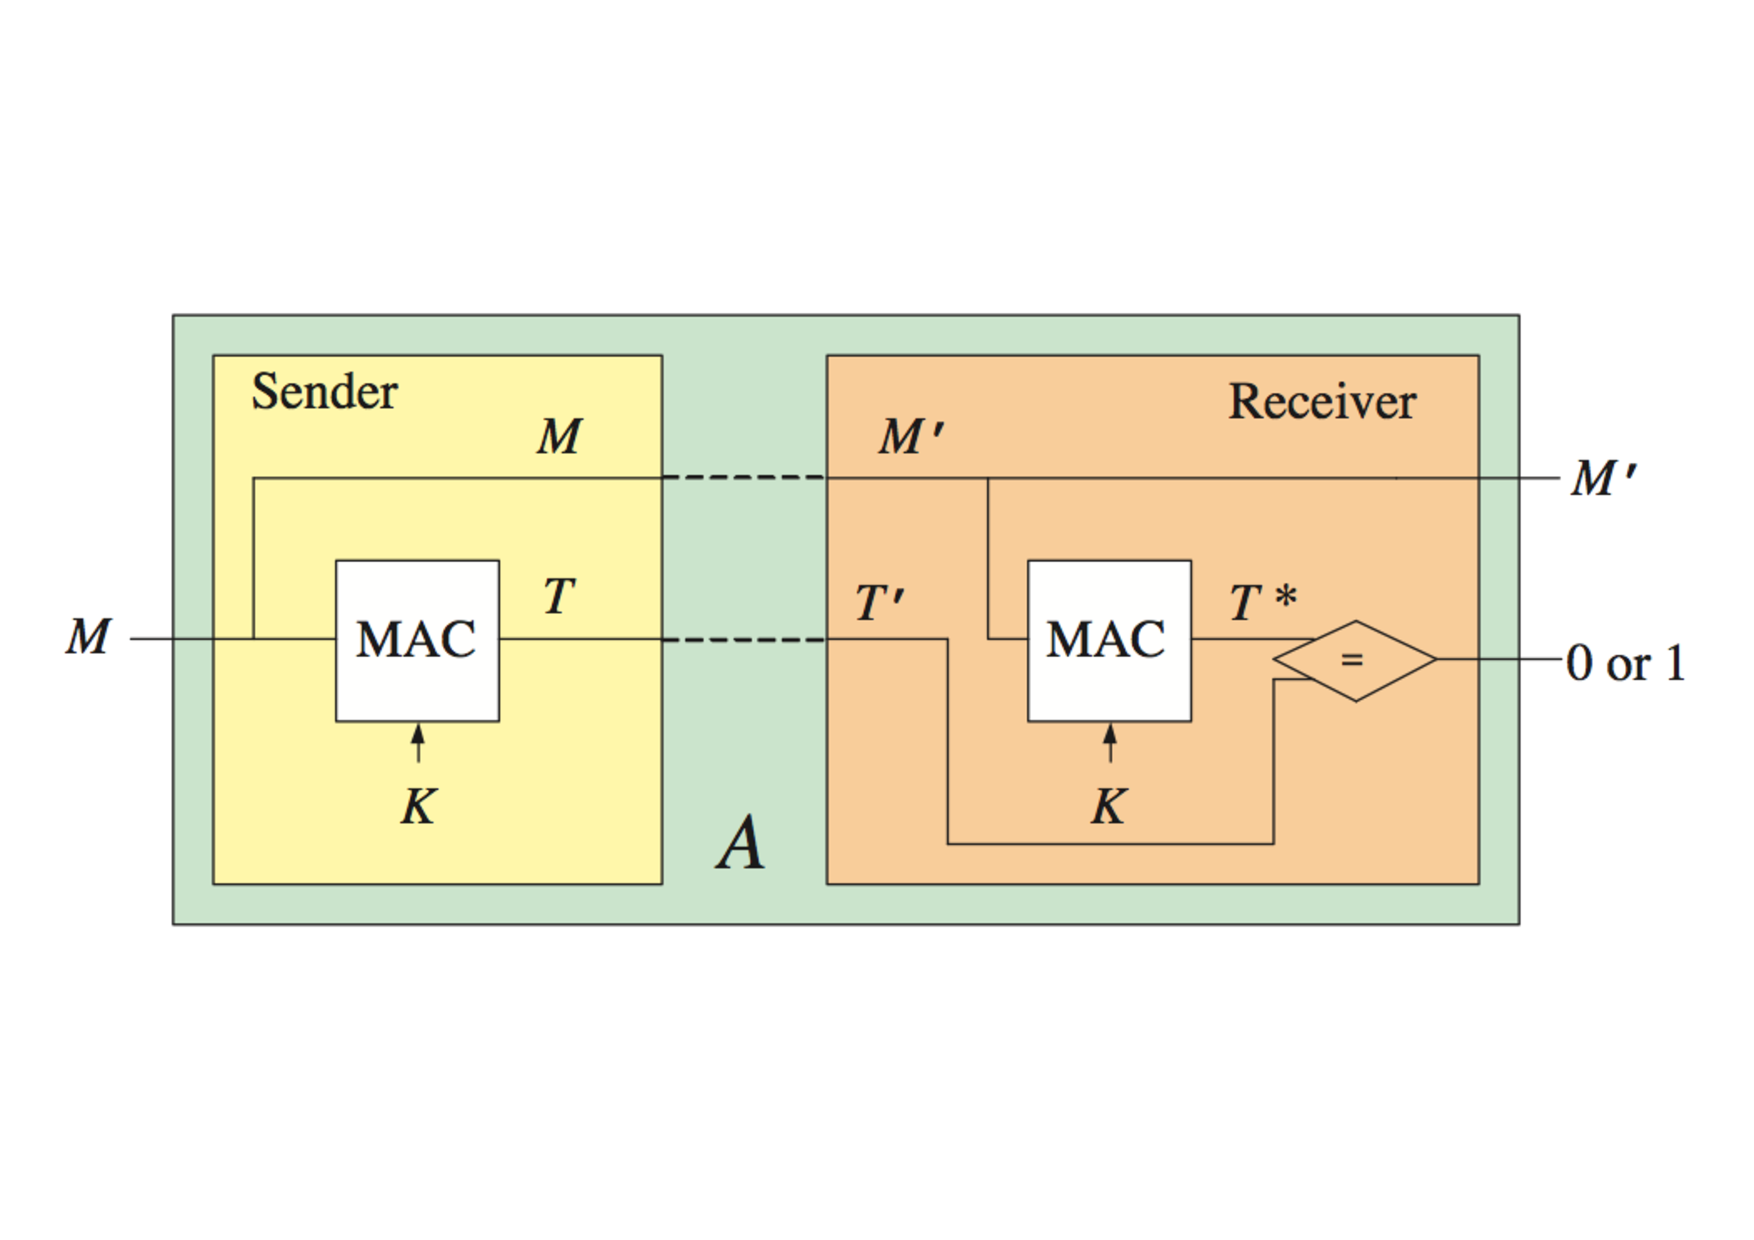
\includegraphics[scale=0.4]{./diagrams/MAC.pdf}
\caption{The Concept of Deterministic MAC Scheme}
\label{deterministic_mac }
\end{figure}
Message Authentication Code(MAC), called tag in some research works, is a short message block. A tag is generated by a MAC scheme by accepting a data block D as input and process D with a secret key K inside the scheme. Some MAC schemes require an additional input block, named nonce, in the generation of tag.  

When the processor writes a data block D to the memory, MAC scheme computes a tag  and concatenate the tag withe data forming a data-tag pair. The data-tag pair is sent to off-chip memory for storage.
When the processor reads a data from memory, the data-pair is sent to the chip and to MAC scheme. Assume the data part is D and tag part is T1. MAC scheme compute a tag T2 using D T2 is compared with T1. If T1 is identical to T2, D is assumed to be untampered.
 
Figure 3-b expresses the functionality of MAC scheme in integrity protection.

If the integrity of a processor-memory system is protected by MAC scheme, the possible attacks are:
\begin{enumerate}
	\item Modify the content of a data-tag pair
	\item Insert new data-tag pair
	\item Replace the content of a data-tag pair with a copy of data-tag pair from other address
	\item Replace the content of a data-tag pair with a copy of this pair in an old time point
\end{enumerate}
If a MAC scheme is capable to defend the 1st and 2nd attacks in the list, it should ensure that for any data block D, the tag is randomly assigned. If this scheme is capable to defend the 3rd and 4th attacks too, it should ensure for any two identical data blocks D1 and D2 that are writen to memory on different time or to different addresses, their tags T1 and T2 should be randomly generated.

\paragraph{Block-level  Added Redundancy Explicit Authentication (AREA)}
When the processor writes a data block D to memory, AREA concatenated a nonce N to D to form a data-nonce pair. This data-nonce pair is encrypted to form a ciphertext block E$_k$(D $\mid$ N). The ciphertext block is stored on off-chip memory.

When the processor reads a data block from memory, the ciphertext block is read to the chip and sent to AREA. After decryption, the nonce part of the pair, marked as N2, is compared to the nonce on-chip that is related to data D, marked as N1. If N1 and N2 are identical, D is assumed to be untampered.

If the integrity of a processor-memory system is protected by AREA, the possible attacks are:
\begin{enumerate}
	\item Modify the content of a E$_k$(D $\mid$ N)
	\item Insert new E$_k$(D $\mid$ N)
	\item Replace the content of a E$_k$(D $\mid$ N) with a copy from other address
	\item Replace the content of a E$_k$(D $\mid$ N) with a copy of this ciphertext block in an old time point
\end{enumerate}
If an AREA system is capable to defend the 1st and 2nd attacks in the list, it should ensure that for any data block D, the nonce is randomly assigned, which makes the cipherter block C=E$_k$(D $\mid$ N) a random value. If this scheme is capable to defend the 3rd and 4th attacks too, it should ensure for any two identical data blocks D1 and D2 that are writen to memory on different time or to different addresses, their nonces N1 and N2 should be randomly generated and make the related C1 and C2 random values.

\subsection{Security Evaluation for Authentication Primitives:the Approaches}
\subsubsection{Computational Provable Security}
\paragraph{The forgery attacks}
When attacking a message authentication system, the adversary try to send a pair(M,T) to the receiver to make VF$_k$(M,T)=1 while M did not originate with the legal sender. The fake pair(M$_f$,T$_f$) that makes VF$_k$(M$_f$,T$_f$)=1 is called a forgery from the adversary. A successful forgery attack indicates that the adversary has made a forgery. 
The purpose of a message authentication system is preventing the receiver to accept the message from unauthorized senders, such as an adversary. The quantitative property of a secure message authentication system is the low probability for an adversary to make a successful forgery attack with the limited resource.
\paragraph{Chosen-message attacks}
A strong type of attack that an adversary can conduct on the message authentication system is the adaptive chosen-message attack, marked as uf-cma. When doing uf-cma, the adversary chooses its own input message M and acquires the relative tag T. The adversary try to find the weakness in the design of message authentication system by analyzing the pairs(M,T) of his choice. The uf-cma provides the adversary with the most capability to succeed in the forgery attack. The probability that an adversary conducts a successful forgery attack after limited times of uf-cma is adopted as the basic quantitative security property of a message authentication in cryptography. This fact was also mentioned in \cite{Rogaway2011}.
\paragraph{The Security Notions of MAC schemes}
The formalised quantitative notion of the security of a MAC scheme was introduced by Bellare et al. in \cite{cbc1994}. This notion follows the security notion of digital signature introduced in \cite{signature}. The successful forgery on a MAC scheme from an adversary A is measured by a experiment called Forgery(MAC,A). In Forgery(MAC,A),  
the adversary A is provided a black-box access to the tag generation system TG$_K$(). When TG$_K$() takes an input message M$_i$, it returns tag T$_i$ to A. A conducts uf-cma by keep sending the message queries M$_i$ and observes the relative tag T$_i$ for limited times. On the other hand, A is provided a black-box access to the verification system VF$_K$(). When A sends a pair(M$_j$,T$_j$) to VF$_K$(), the VF$_K$() computes the tag T of M$_j$ and compares T with T$_j$. If T=T$_j$ then VF$_K$()=1 otherwise 0. If A sends a pair(M,T) that makes VF$_K$() outputs 1 while M has not appeared in the previous queries of uf-cma, then A succeeds a forgery attack and Forgery(MAC,A)=1.

The quantitative security notion of a MAC scheme is forgery probability, expressed as Forgery$_MAC$=Pr[Forgery(MAC,A)=1].
\paragraph{The Correlation between Security and Randomness}
Goldreich, Goldwasser, and Micali asserted in \cite{prf} that any good pseudorandom function(PRF) is a secure MAC scheme under the quantitative security notion. Bellare, Kilian and Rogaway proved this assertion in \cite{cbc1994} saying that if a system behave like a pseudoranom function, this system is a secure MAC scheme if meeting the requirements on domain and range of MAC schemes. Based on these two reduction of security notion, latter researches on security evaluation of MAC schemes posted their focuses on analyzing whether the MAC scheme evaluated behaves like a PRF.
\paragraph{The Randomness of a MAC scheme}
The definition of PRF was introduced in \cite{prf} indicating that PRF could not be distinguished from a ideal random function each bit of whose output was a coin flip. To define how closely a MAC scheme behaves like a PRF, Bellare et al. provided a quantitative notion in \cite{cbc1994} named Adv$^{PRF}_{MAC}$(), which was based on the concept of distinguisher introduced in\cite{prf}. 

Let F$_0$ and F$_1$ be two function with a common domain D and a common range R. A distinguisher A for F$_0$ versus F$_1$ is an adverary A that has access to a black box named oracle f:D->R. After accessing the oracle f, A computes a bit. Assume the function stored in the oracle f is X and A guesses that X is in the oracle, then A computes 1 otherwise 0. The the advantage of A in distinguishing F$_0$ from F$_1$ is expressed as Adv$^{F0}_{F1}$=Pr[f$\stackrel{R}{\longleftarrow}$F0:A$^{F0}$=1]-Pr[f$\stackrel{R}{\longleftarrow}$F1:A$^{F1}$=1]. Pr[f$\stackrel{R}{\longleftarrow}$F0:A$^{F0}$=1] means when the content of oracle f is F0, A guesses that F0 is in oracle then output 1.

We can see that if F0 behaves much like F1, it is hard for A to distinguish between F0 and F1 then Adv$^{F0}_{F1}$ is very small. This case is adopted by Bellare et al. in the quantitative notion of randomness of a MAC scheme. If the randomness of a MAC scheme is good, then the MAC scheme behaves like a PRF and Adv$^{[PRF]}_{MAC}$ is small. 

\subsubsection{Formal Method based Evaluation}
\subsubsection{Automated Sound Security Evaluation}


\subsection{Design Works of Authentication Primitives}
\paragraph{What to say in this subsection}
\begin{itemize}
	\item For each type of AP, the designs
	\item For each design, the security analysis and result
\end{itemize}
\subsubsection{Cryptographic Hash Functions}
\subsubsection{Message Authentication Code(MAC) Scheme}
\subsubsection{Block-level Added Redundancy Explicit Authentication (AREA)}

\subsection{Message Authentication(MA) Systems:: the Implementation of Theoretical Model}
\paragraph{What to say in this subsection}
\begin{itemize}
	\item The MA system design
	\item For each MA system, the security analysis and result
\end{itemize}
\paragraph{Concepts of Message Authentication(MA) System}
The purpose of message authentication, marked as MA, is to monitor the integrity of message blocks in the communication. In the scenario of processor-memory communication, MA can be defined as the process to verify that whether "the data read from memory by the processor (or by a specific application) at a given address is the data it last wrote at this address"(\cite{hm_survey}). The on-chip data is assumed to be inaccessible and secure, which is called trusted area; while the data in the transmission and stored in off-chip memory is considered to be accessible to attackers and vulnerable. Transmission path(such as bus) and off-chip memory are called malicious area. 
B\begin{figure}[htbp]
\centering
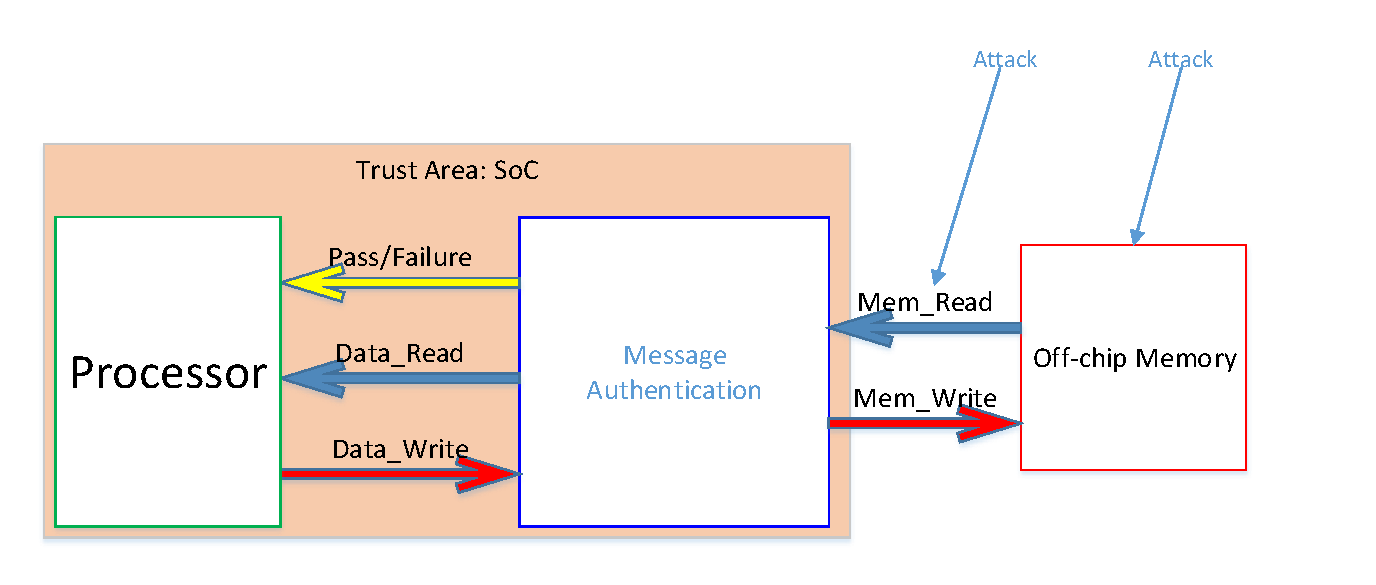
\includegraphics[scale=0.5]{./diagrams/MA_concept.pdf}
\caption{The Concept of MA System}
\label{ma_system}
\end{figure}

Figure 1 expresses the concept of MA for processor-memory communication. 
When processor writes a data block, marked as D, to and address, marked as addr, on the memory, processor sends D to MA system and output a message block, marked as message(D, add$_B$), where add$_B$ represents an additional data block. The message block message(D,add$_B$) can be the data block D only, D concatenated with a short block(commonly called tag) or other format of D. The content of message(D,add$_B$) is determined by the crypographic primitive adopted by the MA system.
When the processor wants to read the data D from address addr, the message(D,add$_B$) is read to SoC and sent to MA system first. After verified by MA, if the data D is not tampered, MA sends a signal indicating pass to processor and send the D to the processor, where D is extracted from message(D,add$_B$) block read from memory.
If the MA finds that the D is tampered, MA sends a failure signal to processor, and invoke the exception handling procedure.
\subsubsection{Hash Function Based MA Systems}
\paragraph{Uniprocessor System}
\paragraph{Multiprocessor System}
\subsubsection{MAC Function Based MA Systems}
\paragraph{Uniprocessor System}
\paragraph{Multiprocessor System}
\subsubsection{Block-level AREA Based MA Systems}
\paragraph{Uniprocessor System}
\paragraph{Multiprocessor System}
\end{document}